\documentclass[xcolor=dvipsnames]{beamer}
\usepackage[utf8]{inputenc} 

\definecolor{LightGray}{gray}{0.75}

\usepackage{textcomp}

\usepackage{caption}

\usepackage{anyfontsize}

\usepackage[font=itshape]{quoting}
\quotingsetup{vskip=4pt} % vertical spacing of quotes


\usecolortheme{seahorse} %colour theme, cf https://www.hartwork.org/beamer-theme-matrix/

\title[] {Group 1.2 - Predicition App}
\date{} % no date

% empty to have to numbering of split-up frames from allowframebreaks
% cf http://tex.stackexchange.com/questions/193308/how-can-we-change-allowframebreaks-numbering-in-the-title#212292
\setbeamertemplate{frametitle continuation}{}


\begin{document}

\frame{\titlepage}

\begin{frame}
	\frametitle{Workflow}
	\includegraphics[width=\textwidth]{tasks.png}
\end{frame}

\begin{frame}
	\frametitle{What we have achieved so far - Design}
	%
	\large{Milestone 1 (15.5.)}
	\normalsize
	\begin{itemize} 
		\item \color{Green}Grundliegende Software-Architektur festgelegt
		\item \color{Green}Grundliegendes Software-Design festgelegt
		\item \color{Green}Ein Grundgerüst der Applikation ist fertiggestellt: Es sind folgende Ansichten funktional umgesetzt:
		\begin{itemize} 
			\item \color{Green}Offline-Karten (eine Kartenumgebung wird angezeigt, Navigation möglich)
			\item \color{Green}Diverse UI-Elemente (mindestens Eingabefeld, Button)
		\end{itemize} 
		\item \color{LightGray}Die Positionsdaten für die Vorhersage werden von der \textit{Movebank}-API bezogen.
	\end{itemize}     
	%
	\large{Milestone 2 (5.6.)}
	\normalsize
	\begin{itemize} 
		\item \color{LightGray}Es wird eine Vorhersage mittels eines einfachen Vorhersagemodells berechnet.
		\item \color{LightGray}Es existiert eine funktionale Visualisierung des Vorhersage-Ergebnisses.
		\item \color{LightGray}Es existiert eine Möglichkeit, eine Cesium Ansicht von der Applikation aus aufzurufen.
		\item \color{Green}Der Aufbau des User-Interfaces ist festgelegt (nicht-funktionale Mockups).
	\end{itemize}
\end{frame}



\begin{frame}
	\frametitle{What we have achieved so far - Movebank}
	\Large{Milestone 1 (15.5.)}
	\normalsize
	\begin{itemize} 
		\item \color{LightGray}Grundliegende Software-Architektur festgelegt
		\item \color{LightGray}Grundliegendes Software-Design festgelegt
		\item \color{LightGray}Ein Grundgerüst der Applikation ist fertiggestellt: Es sind folgende Ansichten funktional umgesetzt:
		\begin{itemize} 
			\item \color{LightGray}Offline-Karten (eine Kartenumgebung wird angezeigt, Navigation möglich)
			\item \color{LightGray}Diverse UI-Elemente (mindestens Eingabefeld, Button)
		\end{itemize} 
		\item \color{Green}Die Positionsdaten für die Vorhersage werden von der \textit{Movebank}-API bezogen.
	\end{itemize}     
\end{frame}




\begin{frame}
	\frametitle{What we have achieved so far - Database}
    

    
\end{frame}



\begin{frame}
	\frametitle{What we have achieved so far - Algorithms I}
	%
	\large{Milestone 2 (5.6.)}
	\normalsize
	\begin{itemize} 
		\item \color{Green}Es wird eine Vorhersage mittels eines einfachen Vorhersagemodells berechnet.
		\item \color{LightGray}Es existiert eine funktionale Visualisierung des Vorhersage-Ergebnisses.
		\item \color{LightGray}Es existiert eine Möglichkeit, eine Cesium Ansicht von der Applikation aus aufzurufen.
		\item \color{LightGray}Der Aufbau des User-Interfaces ist festgelegt (nicht-funktionale Mockups).
	\end{itemize}
\end{frame}

\begin{frame}
	\frametitle{What we have achieved so far - Algorithms II}
	\Large{AlgorithmExtrapolationExtended}
	\normalsize{}
			\begin{itemize}
				\item[(+)] Good if the variance of the angles is not too big
				\item[(+)] Later datapoints are weighted more
				\item[(+)] Fast
				\item[(+)] Easy to understand
				\item[] 
				\item[( - )] Not very accurate
				\item[( - )] Early data gets ignored

			\end{itemize}
\end{frame}

\begin{frame}
	\frametitle{What we have achieved so far - Algorithms III}
	\Large{AlgorithmSimilarTrajectory}
	\normalsize{}
			\begin{itemize}
				\item[(+)] Good if the measuring frequency is high
				\item[(+)] Earlier datapoints are important for the result
				\item[(+)] Multiple trajectories can be found
				\item[(+)] Easy to understand
				\item[] 
				\item[( - )] Frequency is not always high $\Rightarrow$ Wrong result
				\item[( - )] Higher complexity than the other algorithm
				\item[( - )] (Currently) only works with the same time span between datapoints
			\end{itemize}
\end{frame}



\begin{frame}
	\frametitle{What we have achieved so far - Visualization (OSM) I}
	%
	\large{Milestone 2 (5.6.)}
	\normalsize
	\begin{itemize} 
		\item \color{LightGray}Es wird eine Vorhersage mittels eines einfachen Vorhersagemodells berechnet.
		\item \color{Green}Es existiert eine funktionale Visualisierung des Vorhersage-Ergebnisses.
		\item \color{LightGray}Es existiert eine Möglichkeit, eine Cesium Ansicht von der Applikation aus aufzurufen.
		\item \color{LightGray}Der Aufbau des User-Interfaces ist festgelegt (nicht-funktionale Mockups).
	\end{itemize} 
	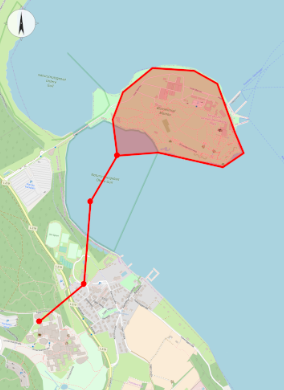
\includegraphics{VisualizationFunctional.png}
\end{frame}


\begin{frame}
	\frametitle{Next steps - Visualization (OSM) II}
	%
	\begin{itemize} 
		\item Design suitable visualizations for different types of\\ prediction output (trajectories, clouds, ...)
		\item Display current location
	\end{itemize} 
\end{frame}


\begin{frame}
	\frametitle{What we have achieved so far - Visualization (Cesium)}
	%
	\large{Milestone 2 (5.6.)}
	\normalsize
	\begin{itemize} 
		\item \color{LightGray}Es wird eine Vorhersage mittels eines einfachen Vorhersagemodells berechnet.
		\item \color{LightGray}Es existiert eine funktionale Visualisierung des Vorhersage-Ergebnisses.
		\item \color{Green}Es existiert eine Möglichkeit, eine Cesium Ansicht von der Applikation aus aufzurufen.
		\item \color{LightGray}Der Aufbau des User-Interfaces ist festgelegt (nicht-funktionale Mockups).
	\end{itemize} 
\end{frame}






\end{document}